\newpage
\section{Validation}
\begin{definition}
    Definiamo \textbf{selezione del modello} la stima delle prestazioni (generalizzazione errore) di diversi modelli 
    di apprendimento al fine di scegliere il migliore (per generalizzare).
\end{definition}
\hspace{-15pt}Questo include la ricerca dei migliori iperparametri del tuo modello (es. ordine polinomiale, lambda di regressione di cresta, ...)
\begin{definition}
    Definiamo come \textbf{valutazione del modello} quando dopo aver scelto uno modello finale, si va a stimare/valutare il proprio
    errore/rischio di previsione (generalizzazione errore) su nuovi dati di test (misura della qualità/prestazione del modello scelto alla fine).
\end{definition}
\subsection{Hold out}
Una regola molto importate è quello di mantenere la separazione tra gli obiettivi e utilizzare set di dati separati in ogni fase.\\
Se la dimensione del set di dati è sufficiente, per esempio $50\%$ TR, $25\%$ VL, $25\%$ set disgiunti.
\begin{figure}[h!]
    \centering
    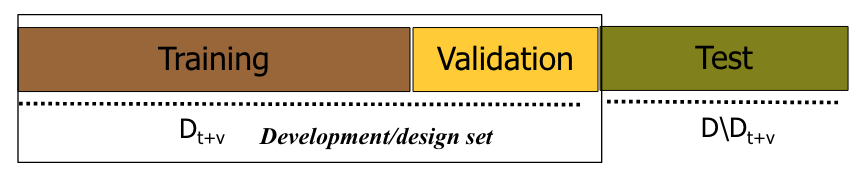
\includegraphics[width=0.4\textwidth]{images/validation-hold-out.png}
\end{figure}
\vspace{-5pt}
Vediamo ora quello che chiamiamo \textbf{hold out}:
\begin{itemize}
    \item \textbf{TR}: training set è usato per adattarsi [\textbf{training}]
    \item \textbf{VL}: Validation set (o selection set) è usato per selezionare il miglior modello (fra differenti modelli e/o configurazioni di iperparametri) [\textbf{model selection}]
    \item TR+VL alcune volte sono insieme e vengono chiamate \textbf{insieme di development/design}, usate per costruire il modello finale.
    \item \textbf{TS}: test set è usato per stimare l'errore di generalizzazione (del modello finale) [\textbf{valutazione del modello}] 
\end{itemize}
\begin{note}
    Notare che la stima fatta per la selezione del modello (sul set VL) [è a scopo di selezione del modello], non è una vuona stima per la dase di valutazione/test di rischio. Inoltre
    i risultati del set di test non possono essere utilizzati per la selezione del modello (o chiamarlo set di convalida).
\end{note}
E cosa succederebbe se si usasse il test set in un ciclo di progettazione (ripetuto)?\\
Stiamo effettuando una selezione del modello e una valutazione non affidabile (stima di errore di generalizzazione previsto) e non saremmo in grado di farlo su esempi futuri, concetto di \textbf{set di test cechi} (ad esempio nelle competizione di ML).
In tal caso, l'errore del set di test fornice una valutazione eccessivamente ottimistica per il vero errore del test (vedremo come è facile ottenere una classification accuracy molto alta un un compito casuale anche utilizzando solo il set di test implicito). \\\\
\textbf{Gold rule}: Mantenere la separazione tra gli obiettivi e utilizza set separati in ogni fase (TR per la formazione, VL per la selezione del modello, TS per la stima del rischio)
\begin{figure}[h!]
    \centering
    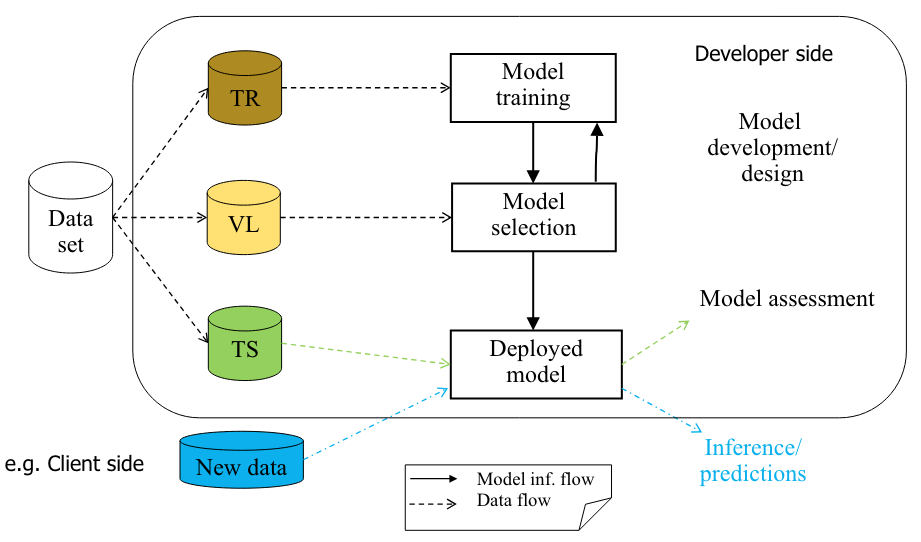
\includegraphics[width=0.52\textwidth]{images/schema-trvlts.png}
\end{figure}
\newpage
\subsection{Un semplice meta-algoritmo}
Vediamo i vari passi di semplice meta algoritmo:
\begin{enumerate}
    \item Separare gli insiemi \textbf{TR} (training), \textbf{VL} (validation) e \textbf{TS} (test).
    \item Cercare il migliore $h_{w,\lambda}()$ modificando gli iperparametri del modello $\lambda$ (es. l'ordine del polinomio, il valore del $\lambda$ per la regressione)
    \item Per ogni diverso valore di $\lambda$ (ricerca in griglia)
    \begin{itemize}
        \item Cerca il migliore $h_{w,\lambda}()$ che minimizzi l'errore/perdita empirica (adattandosi al set TR), trovare i migliori parametri $w$ dove migliore = errore miimo sul set TR (es. $argmin_w Loss(w) \in L_2$) 
    \end{itemize}
    Questo è un doppio ciclo, la ricerca migliore può essere un for loop, per ogni valore $\lambda$ si addestra un modello $h_{w,\lambda}$ (nel ciclo interno, ad esempio il ciclo di discesa del gradiente) e quindi si calcolano i risultati (accuracy) sul set VL.
    Quindi prendi il valore miglior di $\lambda$ ovvero il modello con errore $VL$ minimo o precisione VL massima, ecc.
    \item Selezionare il miglior $h_{w, \lambda}()$: dove migliore = erroe minimo sul set VL.
    \item (Opzionale) Ora è anche possibile adattare $h_{w, \lambda}(x)$ su TR+VL con il miglior modello $\lambda$
    \item Valutare il finale $h_{w, \lambda}$ nel TS.  
\end{enumerate}

\begin{example}
    Vediamo per esempio la ricerca su una griglia con 2 iper-parametri.\\
    Trovare il valore degli iperparametri (ovvero i parametri che non sono direttamente appresi, che non vengono modificati dalla formazione). Il miglior
    iperparametro di ricerca può essere un $<<FOR>>$ su una griglia di valori candidati. Per ogni modello di training $h_{w, \lambda}$ calcolare i risultati (accuracy) sul VL impostato. 
    Quindi prendi quello con l'errore minimo o la precisione massima.
    \begin{figure}[h!]
        \centering
        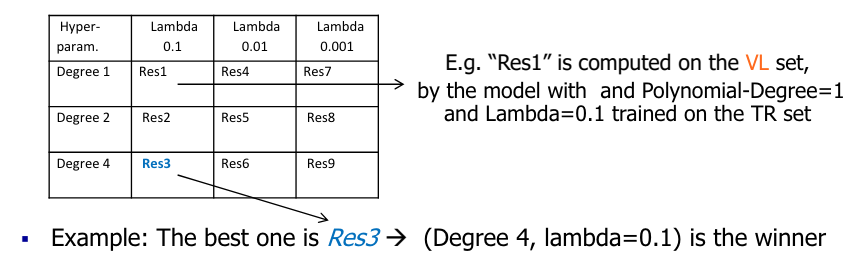
\includegraphics[width=0.5\textwidth]{images/ess-search-on-grid.png}
    \end{figure}

    \hspace{-15pt}Possiamo automatizzarlo. La parallelizzazione è semplice (indipendenza delle prove), esistono alternative
    per ridurre i cosi o automatizzare la ricerca.
\end{example}

\begin{example}
    Vediamo ora un controesempio (separare TR, VR e TL). Abbiamo circa 20-30 esempi, 1000 variabili di input random.
    un \textbf{random} target 0/1. Scelgo 1 modello con una sola variabile/feuture che in indovina 'per caso' al
    $99\%$ sul dataset e poi su qualsiasi split successivo in training, validation e test set.\\\\
    Abbiamo che il valore perdetto $99\%$ non è una buona stima dell'errore di test (quello corretta è $50\%$)
    \begin{enumerate}
        \item Errore stimato su training o validation per model selection NON è utile per stima del rischio! Dati di TR o VL non vanno usati per scopi di test.
        \item Usare tutto il data set per feature/model selection lede la correttezza della stima (risultati biased - $<<$Feature Selection bias$>>$). Test se è stato usato implicitamente dall'inizio.
        Test deve essere separato prima, prima di qualsiasi model selection o design del modello (incluso selezione di features)
    \end{enumerate}
    Un test set esterno fornisce invece la stima corretta del $50\%$ (random coin result). È la \underline{correttezza della stima} che è in giudizio, non la possibilità di risolvere la task.
    \begin{figure}[h!]
        \centering
        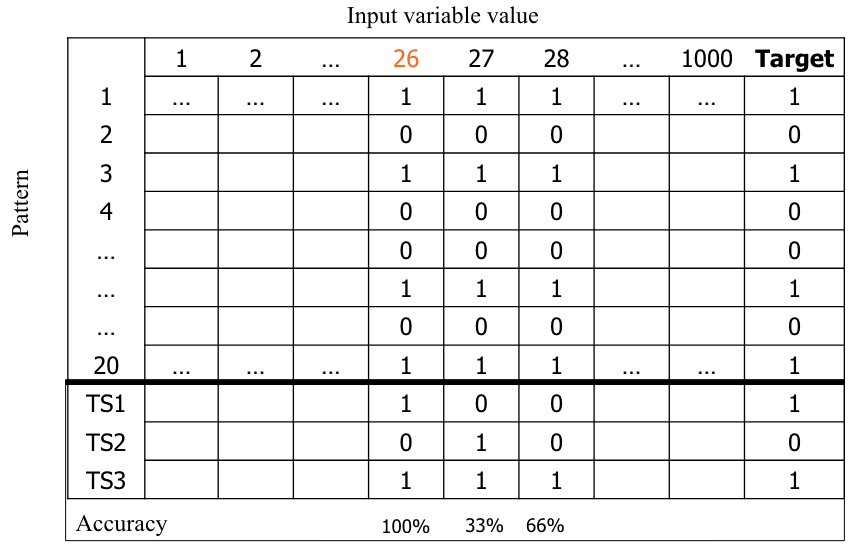
\includegraphics[width=0.6\textwidth]{images/controesempio.png}
    \end{figure}
\end{example}

\subsection{K-fold}
Mantere il CV piò fare un uso insufficiente dei dati.
\begin{definition}
    Definiamo la \textbf{convalida incrociata k-fold} come:
    \begin{itemize}
        \item Suddividere il set di dati D in k sottoinsiemi mutualmente esclusivi $D_1, D_2, \dots, D_k$
        \item Addrestrare l'algoritmo di apprendimento su $D \setminus D_i$ e testarlo s $D_i$
        \item Riassumere la media di tutti i risultati $D_i$ (diagonale)
        \item Utilizza tutti i dati per la formazione, la convalida o il test.
    \end{itemize}
\end{definition}
\begin{note}
    Nota che questa tecnica può essere utilizzata sia per il validation set che per il set di prova.
\end{note}
\hspace{-15pt}Ci sono alcuni problemi di questa tecnica fra qui: decidere quanti "fold", spesso computazionalmente molto costosa, 
abbinabile al set di validazione, doppio k-fold CV, ...
\begin{figure}[h!]
    \centering
    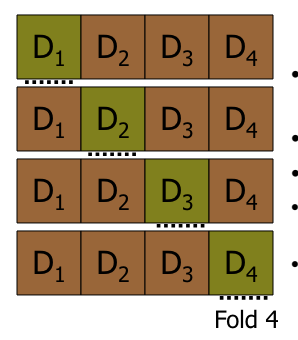
\includegraphics[width=.3\textwidth]{images/hold-out-and-k-fold.png}
\end{figure}
\begin{example}
    Un esempio si selezione del modello e valutazione (con K-fold CV).
    \begin{itemize}
        \item Andiamo a dividere i dati in \textbf{TR} e \textbf{Test set} (qui semplice hold-out o k-fold CV)
        \item \textbf{[Selezione del modello]} Utilizzare k-fold CV (internal) sul set TR, ottenendone di nuovi TR e VL impostati in ogni split, per trovare i migliori iperparametri del tuo modello (es.
        ordine polinomiale, lambda della ridge regression). Questo come?\\
        Andiamo ad applicare una ricerca su gliglia con molti valori possibili dell'iper-parametro. Per esempio:
        un k-fold CV per $\lambda= 0.1$, un k-fold-CV per $\lambda=0.01, \dots$ per poi prendere il migliore $\lambda$ (controntando gli errori medi calcolati sul 
        set di validazione ottenuti da tutte le folds per ogni k-folds CV, il risultato è sulla diagonale dell'immagine).
        \item Allenamento su tutto il TR impostato sul modello finale.
        \item \textbf{[Valutazione del modello]} valutarlo sul l'insieme di test esterno.
    \end{itemize}
\end{example}
Vediamo un tipico comportameto nell'apprendimento.
\begin{figure}[h!]
    \centering
    \begin{subfigure}{0.32\textwidth}
        \centering
        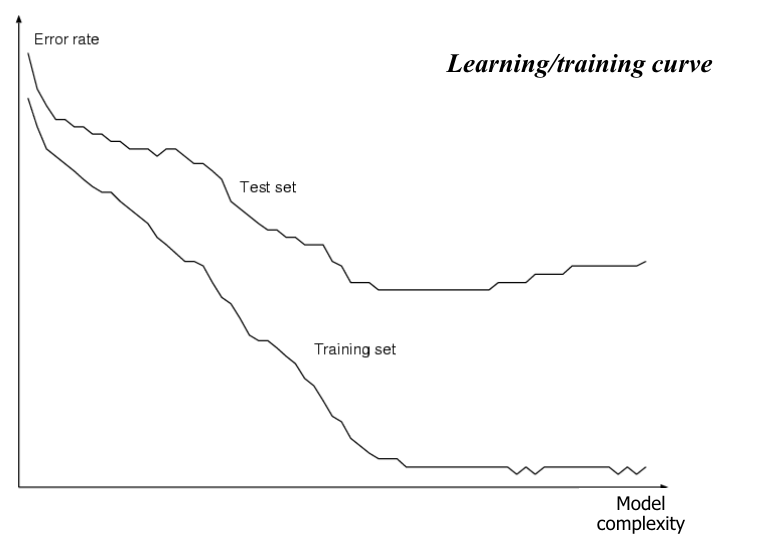
\includegraphics[width=\textwidth]{images/behavior-in-learning-1.png}
    \end{subfigure}
    \begin{subfigure}{0.32\textwidth}
        \centering
        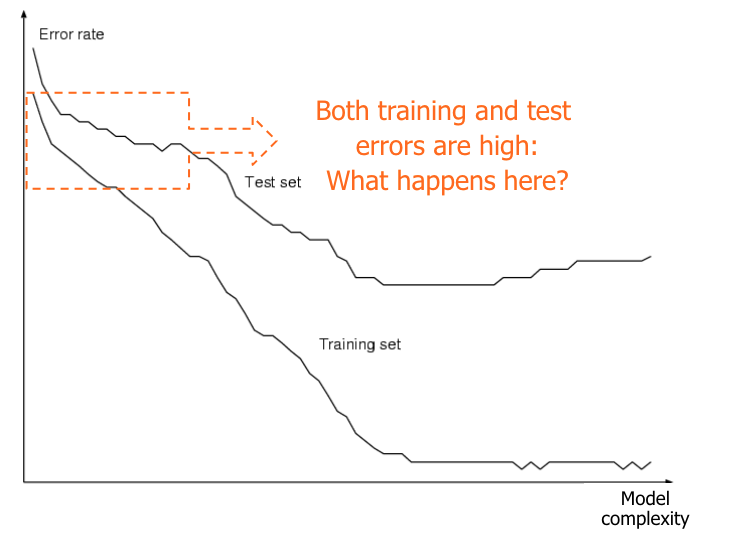
\includegraphics[width=\textwidth]{images/behavior-in-learning-2.png}
    \end{subfigure}
    \begin{subfigure}{0.32\textwidth}
        \centering
        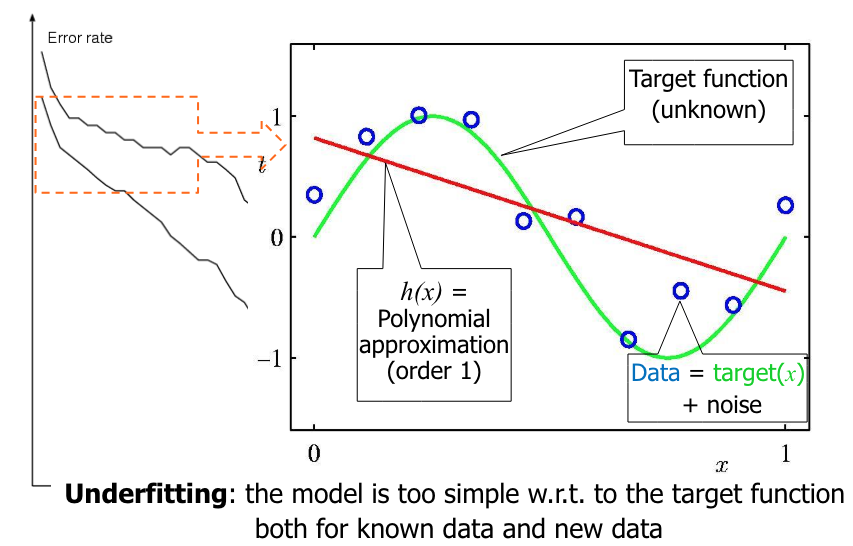
\includegraphics[width=\textwidth]{images/behavior-in-learning-3.png}
    \end{subfigure}
\end{figure}
\begin{figure}[h!]
    \centering
    \begin{subfigure}{0.4\textwidth}
        \centering
        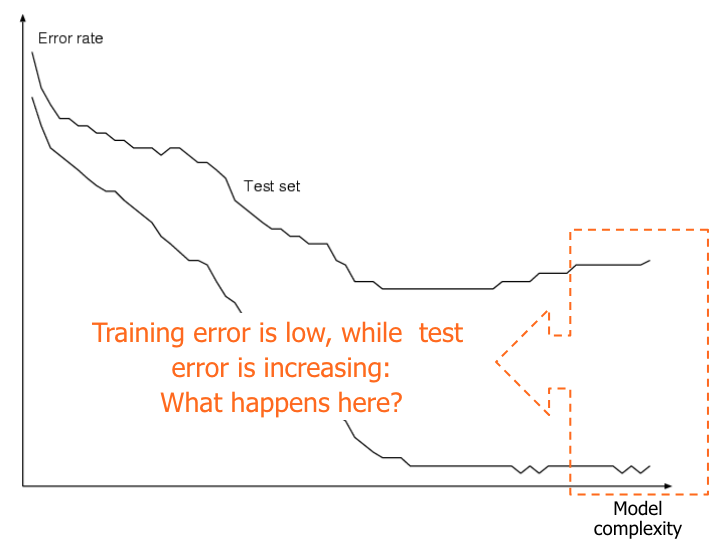
\includegraphics[width=\textwidth]{images/behavior-in-learning-4.png}
    \end{subfigure}
    \begin{subfigure}{0.4\textwidth}
        \centering
        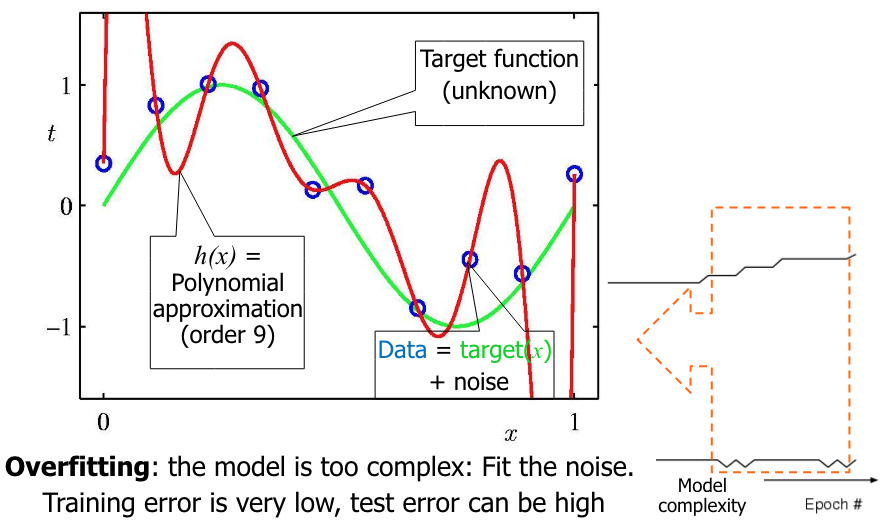
\includegraphics[width=\textwidth]{images/behavior-in-learning-5.png}
    \end{subfigure}
\end{figure}
\begin{figure}[h!]
    \centering
    \begin{subfigure}{0.4\textwidth}
        \centering
        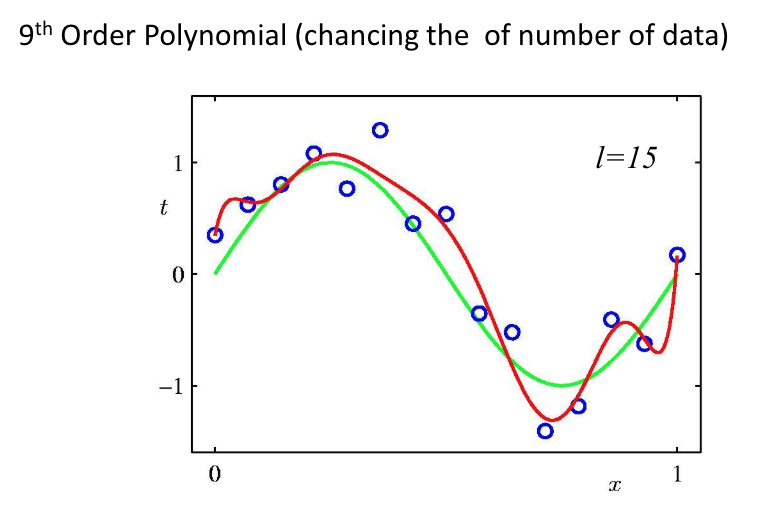
\includegraphics[width=\textwidth]{images/behavior-in-learning-6.png}
    \end{subfigure}
    \begin{subfigure}{0.4\textwidth}
        \centering
        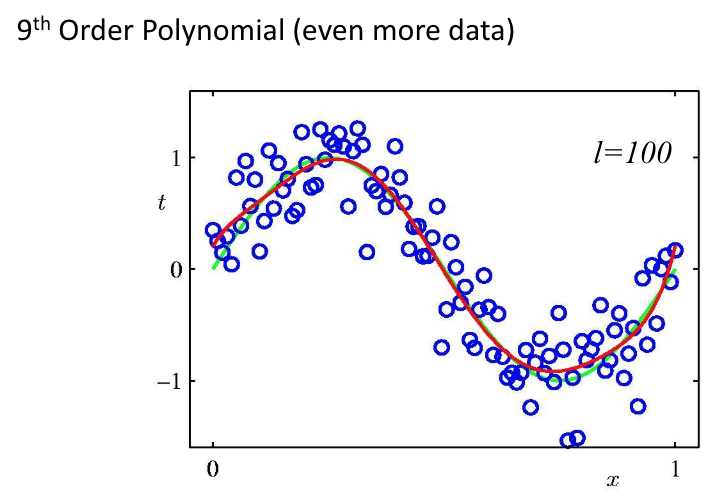
\includegraphics[width=\textwidth]{images/behavior-in-learning-7.png}
    \end{subfigure}
\end{figure}
\subsection{SLT}
Andiamo ora a mettere tutto insieme: la capacità di generalizzazione (misurata come rischio o errore del test) di un modello rispetto all'errore di
formazione o rispetto alle zone di overfitting e underfitting. Poi mettiamo anche insieme il ruolo della complessità del modello, ed il ruolo del numero di dati.
Quello che otteniamo è la \textbf{Teoria di apprendimento statistico} (STL) che è una teoria generale relativa questi argomenti.
\begin{definition}
    Una funzione di approssimazione sconosciuta $f(x)$, $d$ (o $y$, o $t$) è il target ($d=true \: f+noise$). 
    Minimizzare la funzione di rischio: 
    $$R = \int L(d, h(x))dP(x, d)$$
    Dati i valori dall'apprendimento ($d$), la probabilità di distribuzione $P(x, d)$ e una funzione di perdita, ess: $L(h(x), d) = (d - h(x))^2$.\\
    Cercare $h \in H$ che minimizzi $R$. Però non abbiamo solamento l'insieme finito dei dati $TR = (x_p, d_p) \hspace{5pt} p = 1\dots l$. Per cercare $h$
    andiamo a minimizzare il rischio empirico (errore di trining E) frontando il migliori valori per il modello dei parametri liberi.
    $$R_{emp} = \frac{1}{2}\sum_{p=1}^{l}(d_p - h(x_p))^2$$
    Questo si chiama \textbf{principio induttivo della minimizzazione del rischio empirico (ERM)}
\end{definition}
\hspace{-15pt}Possiamo usare $R_emp$ per approssimare R. La risposta è SI ed è stato studiato da Vapnik-Chervonenkis.
\begin{definition}
    Definiamo la \textbf{VC-dim}(VC) come una una misura di complessità dello spazio delle ipotesi
\end{definition}
\begin{definition}
    Definiamo \textbf{VC-bounds} come un limite superiore al rischio. E può essere gestito con una probabilità di $1-\delta$
    $$R \leq R_{emp} + \epsilon(1/l, VC, 1/\delta)$$
    Mente $\epsilon$ si chiama \textbf{VC-confidence}.
\end{definition}
Una prima spiegazione è la seguente:
\begin{itemize}
    \item $\epsilon$ è una funzione che cresce con VC (VC-dim) e descresce con (più alto) $l$ e $\delta$.
    \item Sappiamo che $R_{emp}$ decrementa usando un modello comlesso (con alta VC-dim) (esempio il grado del polinomio)
    \item $\delta$ è la confidenza, regola la probabilità che il bounds varia, roba statistica.
\end{itemize}
L'intuizione è che se abbiamo tanti dati $l$ la VC-confidence si abbassa (tende a 0) ed il rischio empirico $R_{emp}$ va verso $R$.
Se invece ho un modello troppo semplice o rigido (bassa VC-dim) potrebbe essere non sufficiente dovuto al $R_{emp}$ troppo alto (\textbf{underfittig}).
Mente un alto VC-dim, quindi grande complessità del modello, diminuisce il $R_{emp}$ ma la VC-conf, e quindi R, potrebbe aumentare (\textbf{overfitting})\\\\
Per avere la minimizzazione del rischio strutturale bisogna minimizzare il limite!
\begin{figure}[h!]
    \centering
    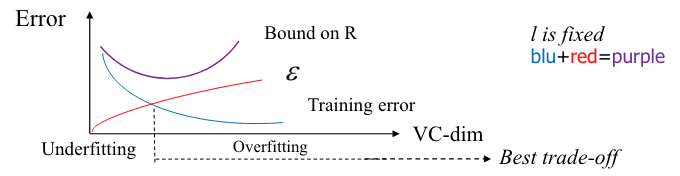
\includegraphics[width=0.6\textwidth]{images/vc-stl-generl-theroy.png}
\end{figure}

\hspace{-15pt}Concetto di controllo della complessità del modello (flessibilià): compromesso tra la TR accuracy (fitting)
e la complessità del modello (VC-dim).\\\\
In sintesi possiamo dire che la SLT permette inquadramento formale del problema della generalizzazione e underfitting/overfitting, 
fornendo limitazioni superiori analitiche e quantitative al rischio R di predizione su tutti i dati, indipendetemnte dal tipo di learning algorithm 
o dettagli del modello.\\\\
Il ML è ben fondato:
\begin{itemize}
    \item Il rischio del learning (e l'errore di generalizzazione) può essere analiticamente limitato, e solo pochi concetti sono fondamentali.
    \item Si può trovare una buona approssimazione dell $f$ target da esempi, pure di avere un buon numero di dati e un'adeguata complessità del modello (misurabile 
    formalmente con la VC-dim)
\end{itemize}
Il STL porta a nuovi modelli (SVM) (e altri metodi che direttamente considerino il controllo della complessità nella costruzione del modello). 
Fonda uno dei principi induttivi sul controllo della complessità.\\\\
Nei modelli lineari la complessità sembra correlata al nuemero di parametri liberi $w$: input dimensione /dim dell'espazione della base (ad esempio grado polinomio).
Parametro lambda per la versione refolarizzata (utilizzando il modello selezione/validazione tecnica per trovare corretto di lambda).
Per il DT invece abbiamo il numero di nodi.